\documentclass[10pt,a4paper]{article}
\usepackage[utf8]{inputenc}

\usepackage{amsmath}
\usepackage{amsfonts}
\usepackage{amssymb}
\usepackage{graphicx}
\usepackage{listings}

\lstset{numbers=left,
	title=\lstname,
	numberstyle=\tiny, 
	breaklines=true,
	tabsize=4,
	language=Python,
	morekeywords={with,super,as},,
	frame=single,
	basicstyle=\footnotesize\tt,
	commentstyle=\color{comment},
	keywordstyle=\color{keyword},
	stringstyle=\color{string},
	backgroundcolor=\color{white},
	showstringspaces=false,
	numbers=left,
	numbersep=5pt,
	literate=
		{æ}{{\ae}}1
		{å}{{\aa}}1
		{ø}{{\o}}1
		{Æ}{{\AE}}1
		{Å}{{\AA}}1
		{Ø}{{\O}}1
	}

\usepackage{bm}
\usepackage{hyperref}
\usepackage[margin=1.25 in]{geometry}
\usepackage[usenames, dvipsnames]{color}

\begin{document}

\begin{center}
{\LARGE\bf
FYS4150\\
Project 3, deadline October 29.
}
 
\includegraphics[scale=0.075]{uio.png}\\
Authors: Robin D. Kifle, Sander W. Losnedahl and Vemund S. Thorkildsen\\
University of Oslo, Autumn 2017

\vspace{3cm}
{\LARGE\bf
Abstract
}

\end{center}

\newpage

{\LARGE\bf
Introduction
}\\

\noindent In this report we will build a model for our solar system. The emphasis will be on creating an object oriented code and calculating the orbits of the planets. The system can be described by using a series of coupled ordinary differential equations. In the first part of the report, a simplified version of the problem will be looked at. This is the hypothetical earth-sun binary situation. Another hypothetical situation will also be looked at, namely a three body system, with Earth, Jupiter and the sun. The equations are rather simple up to three planets, but as the end goal is a system of ten celestial bodies, it will become vital to object orient the code. Preservation of kinetic and potential energy will be discussed, in addition to preservation of angular momentum. The last thing that will be looked upon is the perihelion precession of Mercury. \\

\noindent Two different algorithms will be tested. The euler forward algorithm, and the velocity verlet algorithm. Both of them are numerical integration algorithms, and will be discussed later. The code can be found \href{https://github.com/VemundStenbekkThorkildsen/Assigment3}{\textcolor{blue}{here}}. \\   





{\LARGE\bf
\newpage
Method
}\\

\noindent For the earth-sun binary system, a simple algorithm was made. In this example, the suns position will be fixed. This approximation is okay to make, as the Earth's mass only is three millionths of the suns mass. In this system there is only one force:


$$
F_G=\frac{GM_{\odot}M_{\mathrm{Earth}}}{r^2}
$$

\noindent To use the euler or velocity verlet algorithm, the acceleration must be known. Using newtons second law of motion it it is easy to derive the acceleration. 


$$F_G=M_{Earth}*a $$

$$M_{Earth}*a=\frac{GM_{\odot}M_{\mathrm{Earth}}}{r^2} \Rightarrow a=\frac{GM_{\odot}}{r^2}$$

\noindent Eulers forward method consists of three steps. Firstly the acceleration must be known, as well as initial conditions for position and velocity. As shown above, the acceleration can be calculated easily for this case, but it needs to be decomposed into x- and y-coordinates. 

$$a_x=-G\frac{M_{\odot}}{r^2}cos(\theta)=-G\frac{M_{\odot}x}{r^3}$$
$$a_y=-G\frac{M_{\odot}}{r^2}sin(\theta)=-G\frac{M_{\odot}y}{r^3}$$

\noindent Using that $x=r*cos\theta$ and $y=r*sin\theta$.  The three steps shown for x:

$$a_t=\frac{F_G}{M_{Earth}}$$

$$v_{t+\bigtriangleup t}=v_t + a_t\bigtriangleup t $$

$$x_{t+\bigtriangleup t}=x_t + v_{t+\bigtriangleup t}\bigtriangleup t$$

\noindent The same algorithm applies for y. This algorithm is simple, and only consists of $5n$ FLOPS, but this has its effects on the accuracy. The velocity verlet algorithm can be summarized in four steps. Once again, the algorithm is viable for x- and y-dimension.  

$$a_t=\frac{F}{m}$$

$$x_{t+\bigtriangleup t}=x_t + v_t\bigtriangleup t +\frac{1}{2} a_t\bigtriangleup t^2$$

$$a_{t,t+\bigtriangleup t}=a_t + a_{t+\bigtriangleup t}$$

$$v_{t+\bigtriangleup t}=v_t + \frac{a_{t,t+\bigtriangleup t}}{2}\bigtriangleup t$$

\noindent The velocity verlet algorithm uses $11n$ FLOPS, hence is more time consuming than the Euler forward algorithm. The forces acting upon Earth in the three body problem is more complex. In this case, the force acting upon earth from the sun can be described in the exact same fashion. The new element is the gravitational force of Jupiter. 

$$F_{Earth-Jupiter}=G\frac{M_{earth}M_{jupiter}}{d_{Earth-Jupiter}}$$

\noindent where $d_{Earth-Jupiter}$ is the distance between the planets. The sum of forces acting on earth in this problem: 

$$\sum F = F_{Earth-Jupiter}+ F_{Earth-Sun}= M_{earth}G(\frac{M_{jupiter}}{d_{Earth-Jupiter}} + \frac{M_{\odot}}{r^2}) $$

\noindent The same relations act upon Jupiter, but then the mass of Earth is swapped for the mass of Jupiter. The acceleration in all dimensions can be found by dividing with respective masses and decomposing using the relations showed earlier in this chapter. Continuing on this path will only lead to long equations, and headache. Consider the model for the entire solar system. The forces acting upon earth will be the sum of nine gravitational forces. The forces acting upon the remaining nine celestial bodies can also be expressed as the sum of nine gravitational forces. This underlines the importance of object orientation once again.

\noindent By using conservation of energy, we can derive a formula for escape velocity. The initial speed will be equal to the escape velocity $v_e$. At a later state, the planet has escaped and is positioned an infinite distance away from the sun and the speed will be close to zero. We will only account for kinetic energy, $E_k$, and gravitational potential energy, $E_p$. By conservation of energy: 
$$(E_k+E_p)_i = (E_k+E_p)_{\infty}$$
$$\Rightarrow \frac{1}{2}M_{\otimes}v_e^2 + \frac{-GM_{\odot}M_{\otimes}}{r} = 0 + 0$$
$$\Rightarrow v_e = \sqrt{\frac{2GM_{\odot}}{r}} = 2\sqrt{2}\pi \frac{AU}{yr}$$
where $M_{\otimes}$ = mass of Earth, $G$ = the gravitational constant, $M_{\odot}$ = mass of Sun, and $r$ = distance between the Earth and the Sun.

\noindent This project is well suited for an object oriented code since we have planets with given properties, or members in code language, like initial position and velocity as well as mass. Many more members could be assigned to the planet and the code would still work. 
\\
Each planet was made as an object, passing initial values into our body class. This class takes the the initial values and turn them into member variables, making them available to all classes in the code. The solarSystem class takes these member variables and does operations on them, such as calculating energy and force for each integration step. The integration itself is encoded in the verlet class, which actually contains both the Euler forward method and the velocity Verlet method. Which method to use is up to the user. Another feature of the solarSystem class is the printing function where the position, angular momentum, perihelion angle and distance and total energy is printed to .txt files.
\\
The positions and velocities are vectors which are based on the components class. The class most of all allows for vector based operations such that one can define the position and velocities in terms of their spacial components and this makes the vectors much easier to work with. Other vector operations are also possible with this class such as finding the length of vectors, the cross product of vectors and basic algebraic operations.









\newpage
{\LARGE\bf
Results
}\\
\begin{figure} [h]  

\centerline{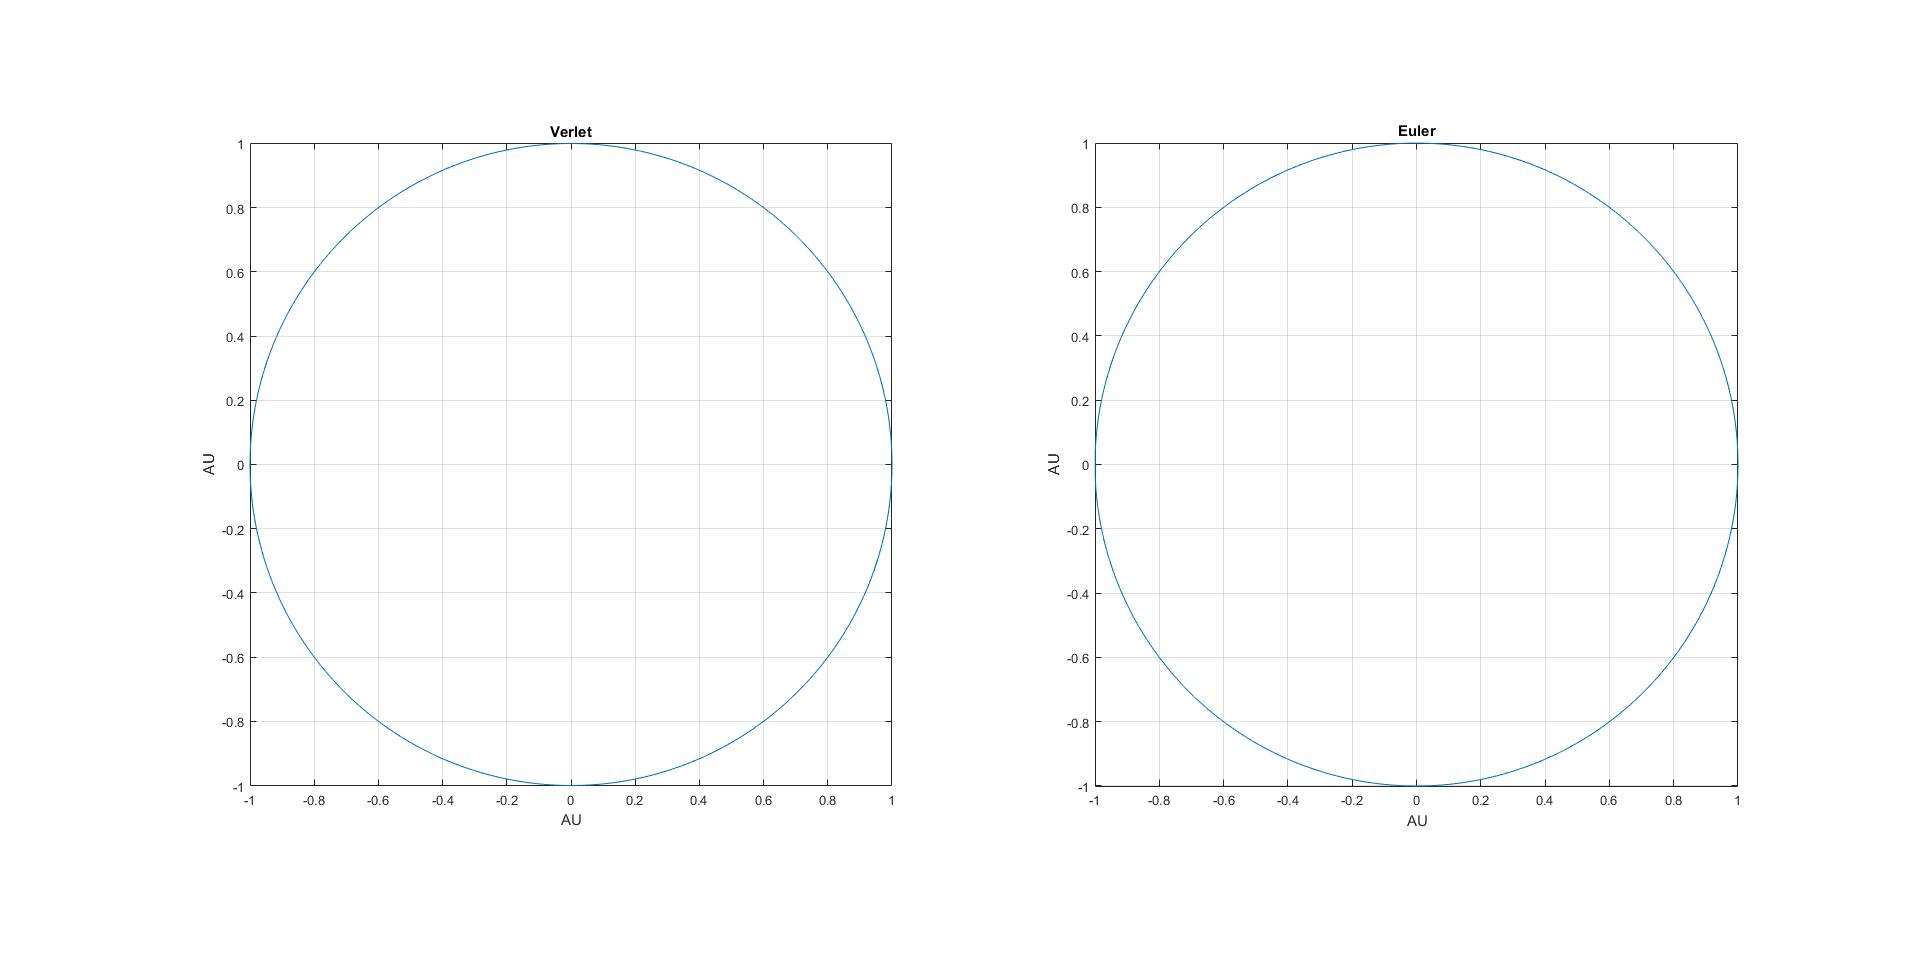
\includegraphics[scale=0.3]{FirstModel.jpg}}
\caption{The planetary orbit of Earth around the sun, with no other interfering forces. Calculated over 100 years with 10000 integration steps per year. This figure was created by using the velocity verlet algorithm}
\end{figure}

\noindent Figure 1 is showing  two models for the Earth-Sun binary system. Both are showing nearly perfect circles, but by playing around with $\bigtriangleup t$, one of the algorithms prove much more solid. As stated earlier, the euler method has fewer FLOPS, but this takes a toll on the accuracy. The velocity verlet algorithm is heavier for the computer to handle, but it gives a much better approximation for each iteration. The kinetic and potential energies should be conserved. 










As there is a circular orbit, there will be small small oscillations in energy. 



\noindent The exact escape velocity of earth was found to be $v=2\sqrt{2}\pi=8.8857$. By trial and error, the escape velocity was found to be $\approx 8.8$, which is pretty close to the actual velocity. 

\begin{figure} [h]  

\centerline{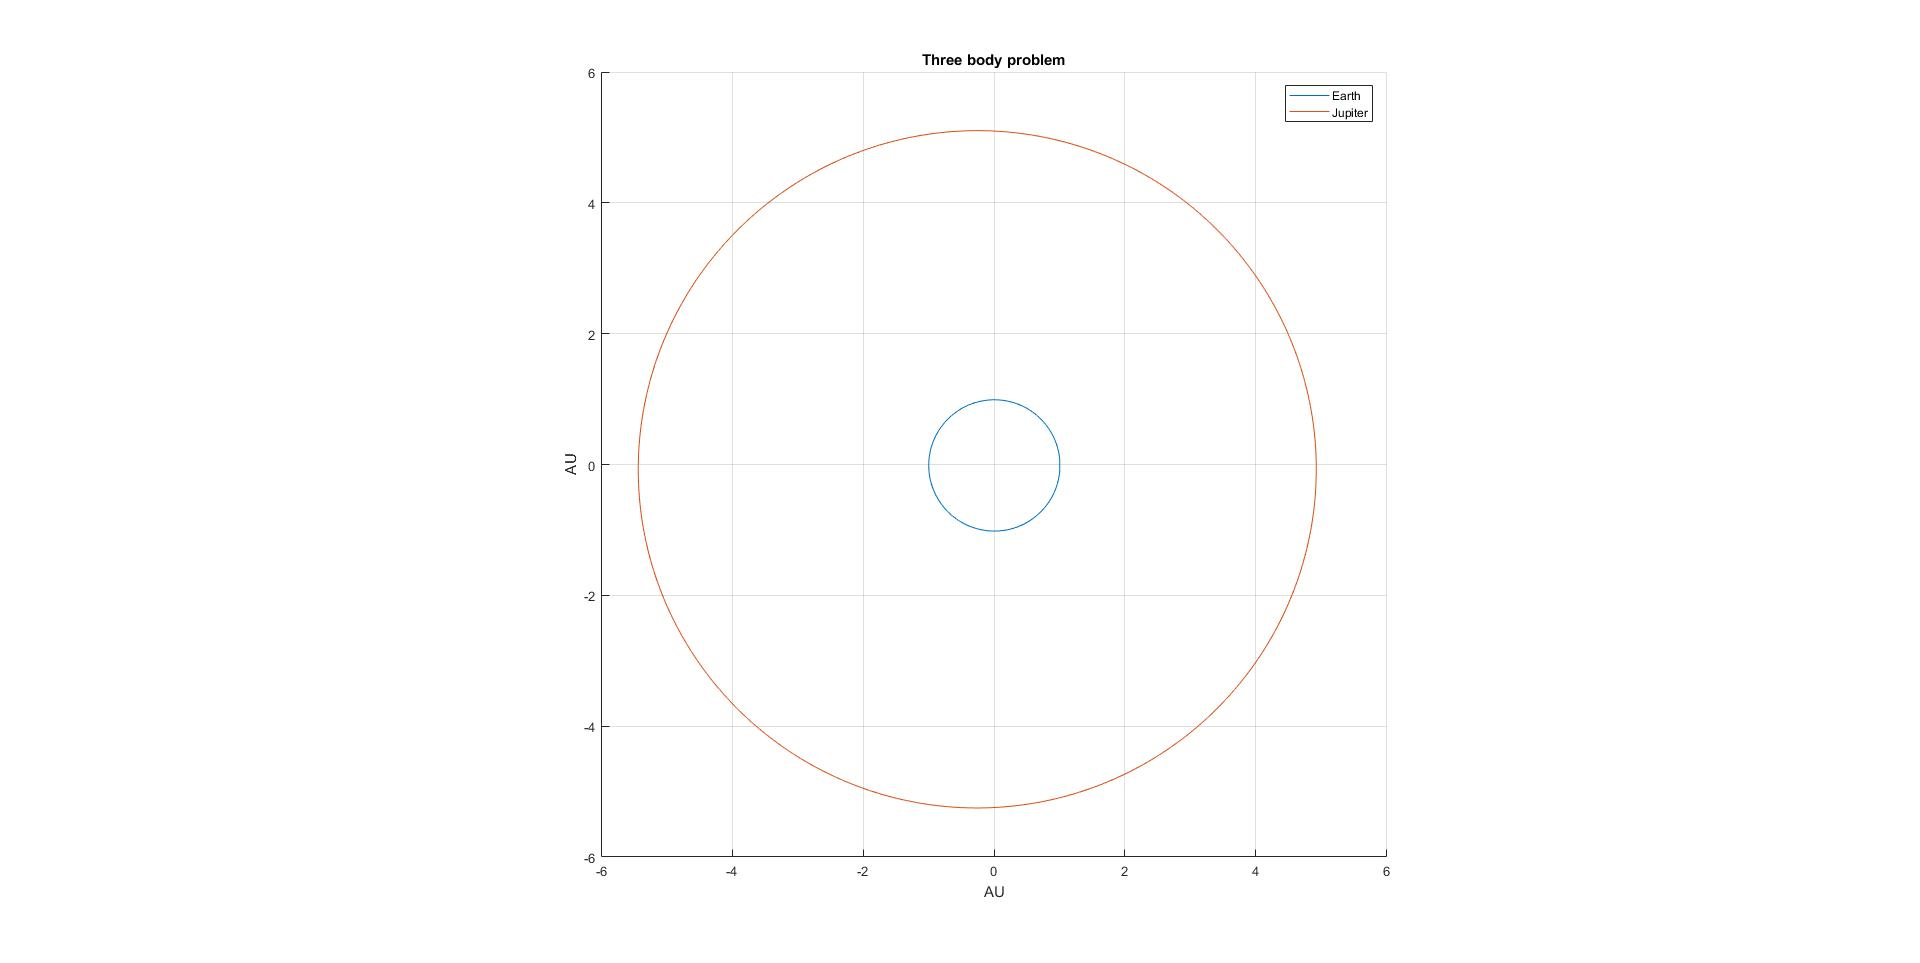
\includegraphics[scale=0.40]{ThreeBody.jpg}}
\caption{The planetary orbits of Earth and Jupiter around the sun, with no other interfering forces. Calculated over 100 years with 10000 integration steps per year.}

\end{figure}



\begin{figure} [h]  

\centerline{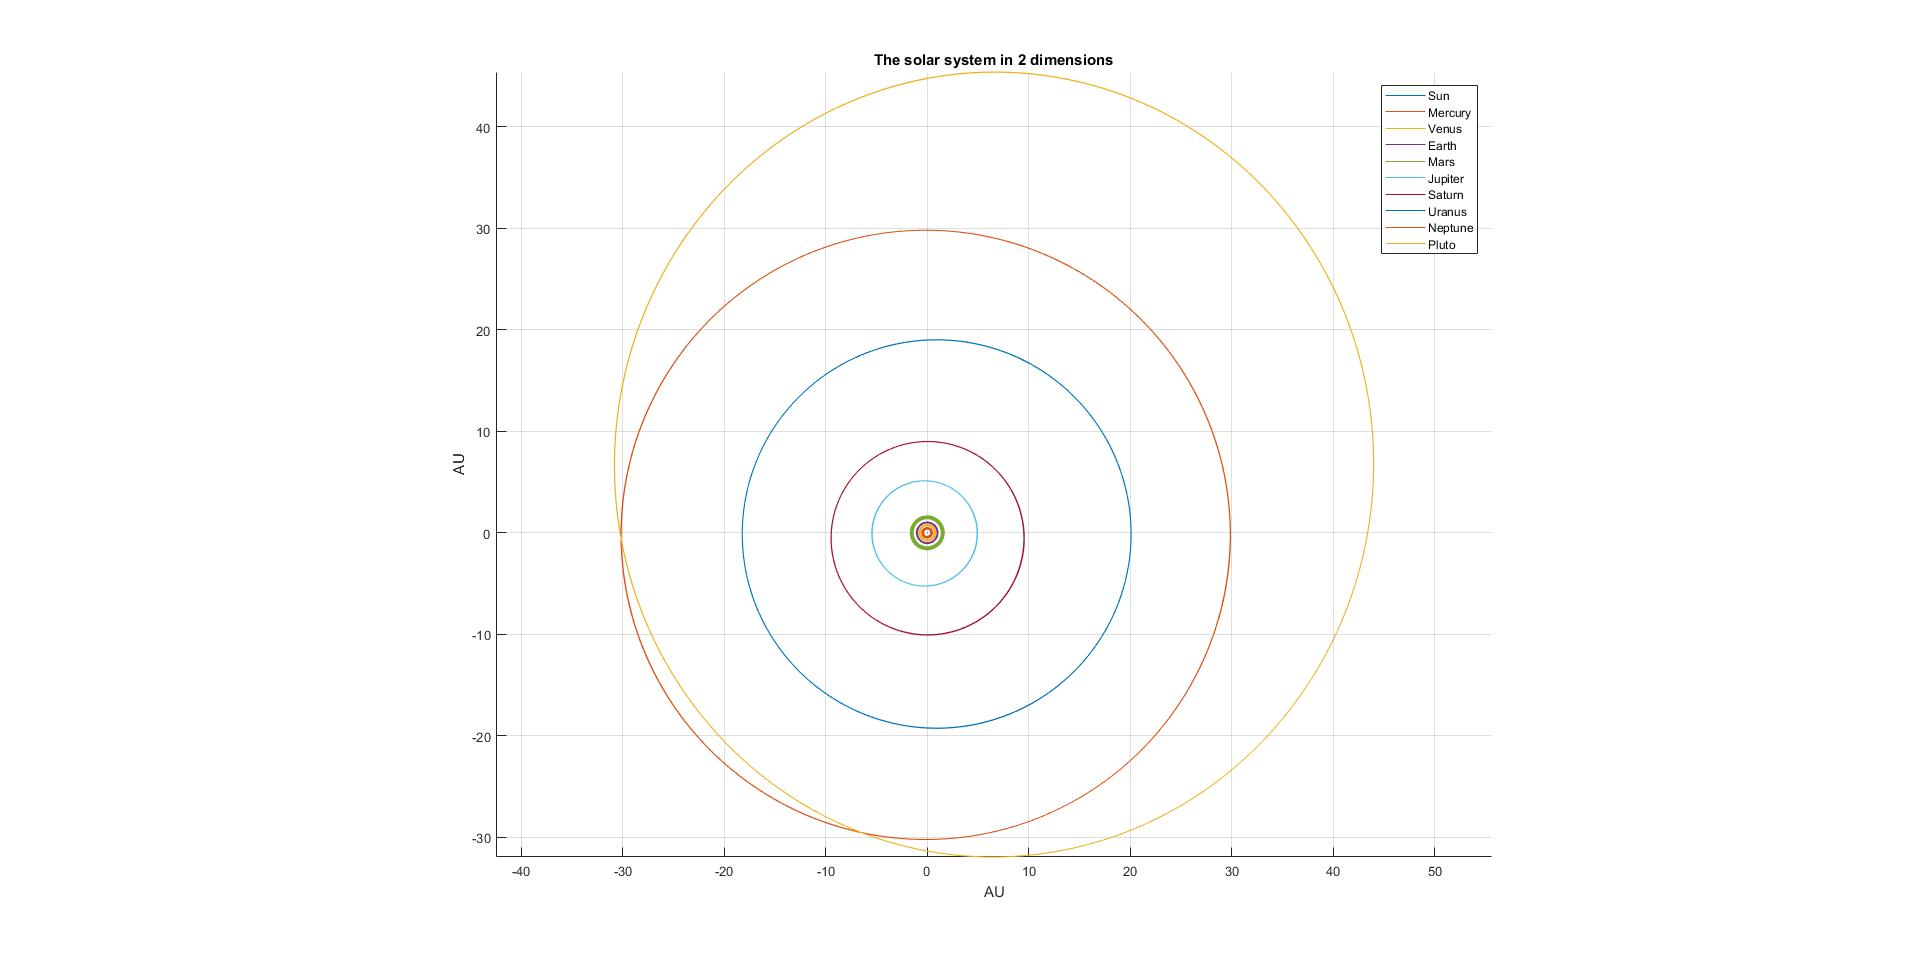
\includegraphics[scale=0.40]{2dsolsys.jpg}}
\caption{The planetary orbits represented in two dimensions for with $10^5$ integration steps over 500 years.}

\end{figure}


\begin{figure} [h]

\centerline{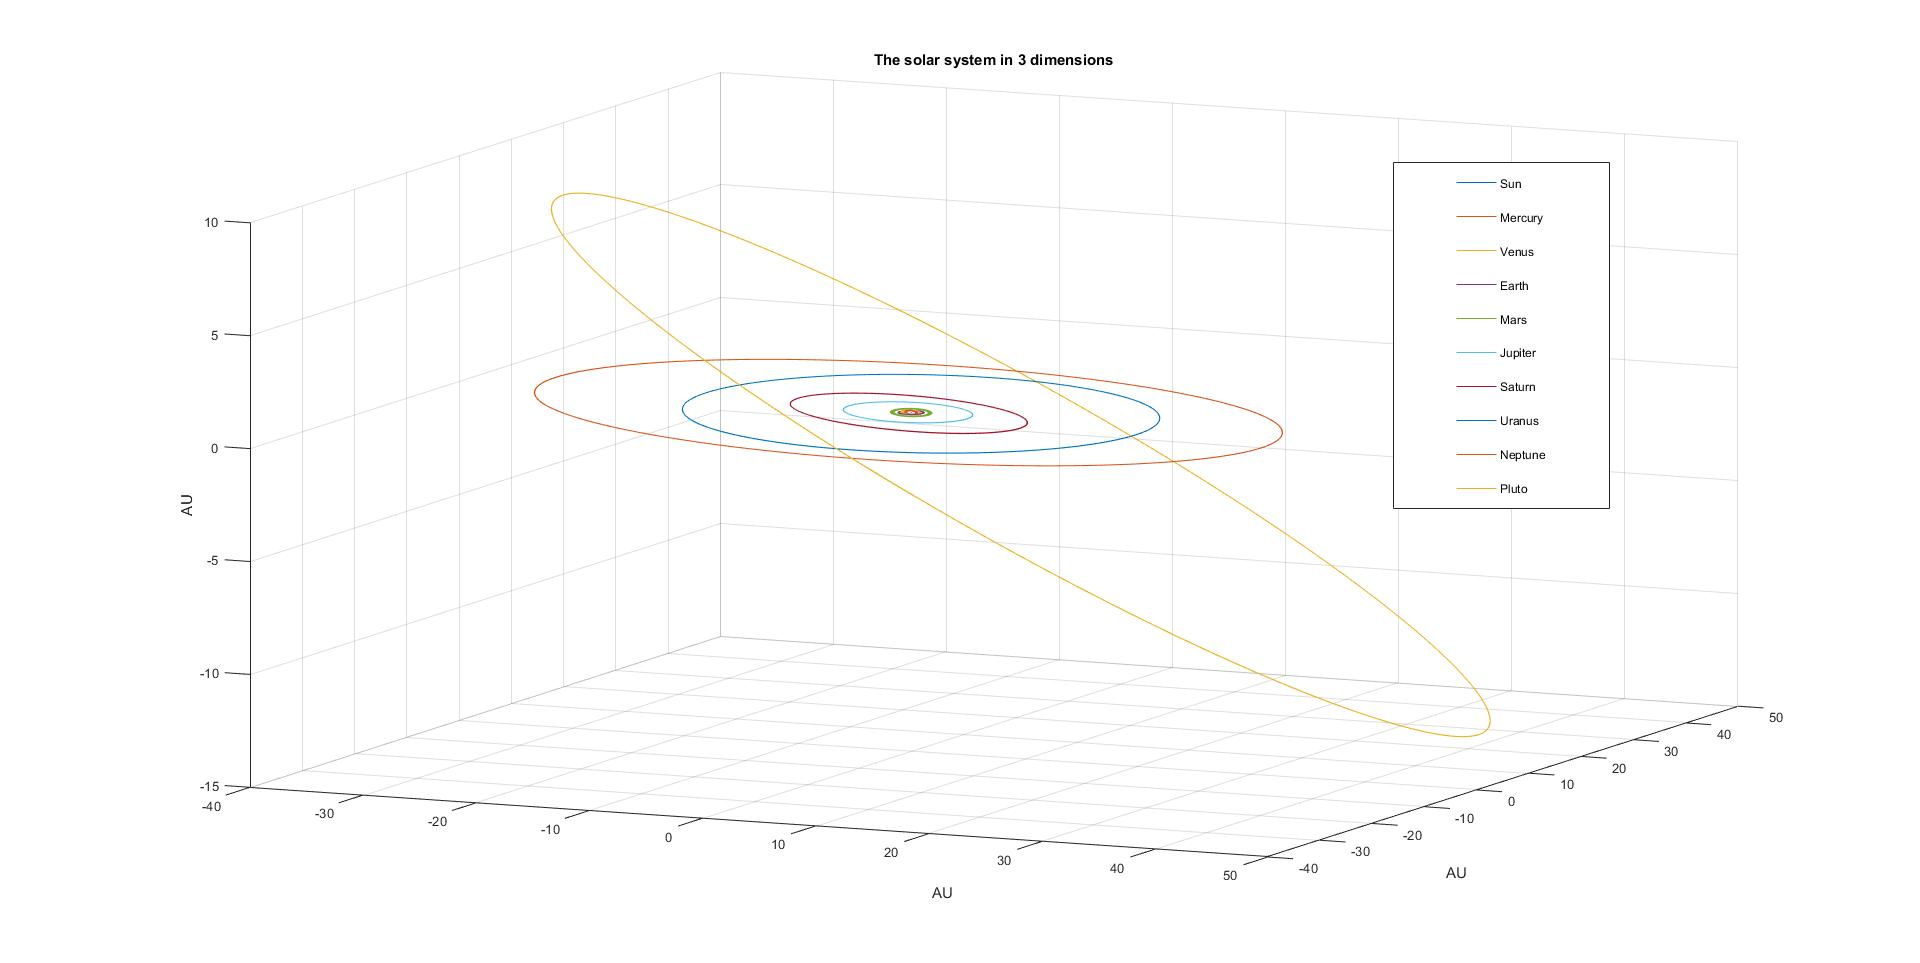
\includegraphics[scale=0.35]{3dsolsys.jpg}}
\caption{The planetary orbits represented in three dimensions for with $10^5$ integration steps over $500$ years.}

\end{figure}



\newpage
{\LARGE\bf
Discussion
}





\newpage
{\LARGE\bf
Conclusion
}









\newpage
{\LARGE\bf
References
}











\end{document}